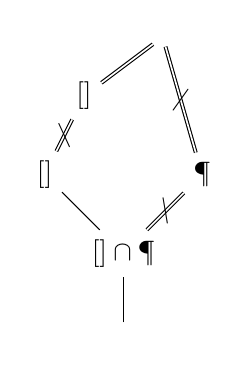
\begin{tikzpicture}
  \node at (0, 0) (nc) {$\NC$};
  \node at (0, 1) (both) {$\NNC[\polylog] \cap \P$};
  \node at (-1, 2) (nncpolylog) {$\NNC[\polylog]$};
  \node at (1, 2) (p) {$\P$};
  \node at (0.5, 3.75) (np) {$\NP$};
  \node at (-0.5, 3) (nnc) {$\NNC[\poly]$};

  \draw (nc) to (both);
  \draw (both) to (nncpolylog);
  \draw[double] (both) -- (p) node[midway, rotate=30] {\small$/$};
  \draw[double] (p) -- (np) node[midway, rotate=-15] {\small$/$};
  \draw[double] (nncpolylog) -- (nnc) node[midway, rotate=45] {\small$/$};
  \draw[double] (nnc) -- (np);
\end{tikzpicture}
